
\chapter{SVM gridsearch}\label{apendix:svm_grid}
    All decision boundary plots for the five best and five worst SVM configurations are found below, sorted by score. As can be seen, all five highest scoring configurations produce a very similar decision boundary.  

    \begin{figure}
        \centering
        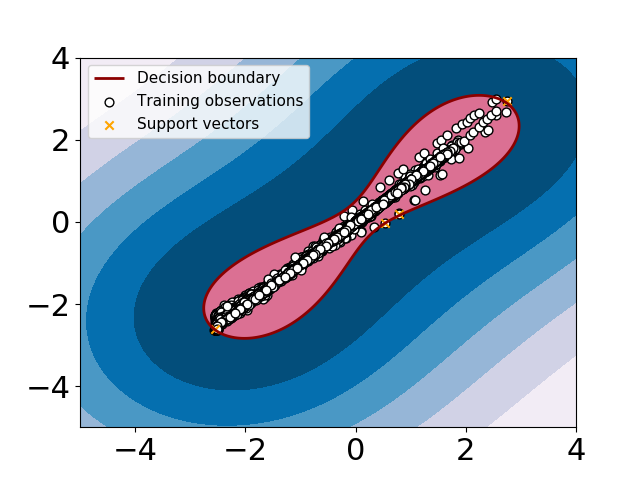
\includegraphics[width = .7\textwidth]{report/figures/analysis/gridsearch/Novelty detection, 1, training, gamma = 0.05 nu = 1.0583130489998942e-05.png}
        \caption{$\gamma = 0.05$, $\nu = 1/N$. score $=0.975$}
        \label{fig:my_label}
    \end{figure}
    
    \begin{figure}
        \centering
        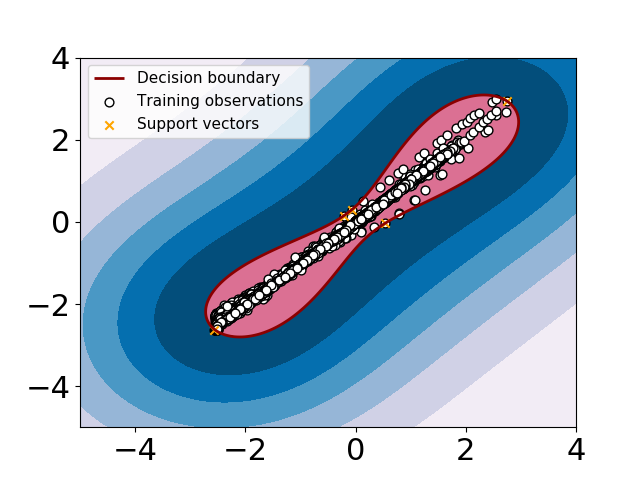
\includegraphics[width = .7\textwidth]{report/figures/analysis/gridsearch/Novelty detection, 2 training, gamma = 0.1 nu = 5.291565244999471e-05.png}
        \caption{$\gamma = 0.1$, $\nu = 1/2N$. score $=0.970$}
        \label{fig:my_label}
    \end{figure}
    
    \begin{figure}
        \centering
        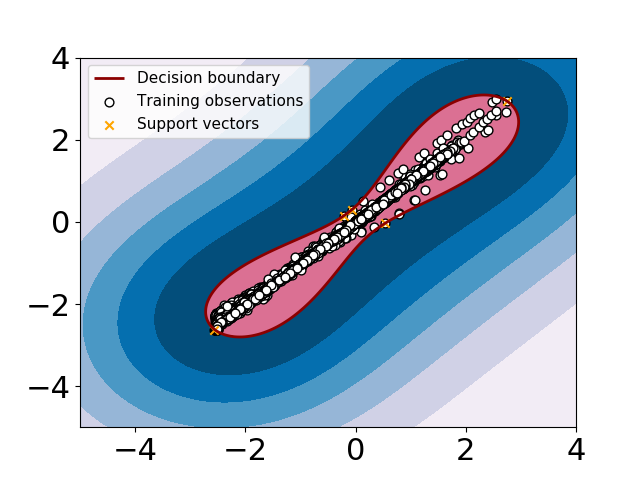
\includegraphics[width = .7\textwidth]{report/figures/analysis/gridsearch/Novelty detection, 3 training, gamma = 0.1 nu = 0.00010583130489998942.png}
        \caption{$\gamma = 0.1$, $\nu = 1/N$. score $=0.961$}
        \label{fig:my_label}
    \end{figure}
    
    \begin{figure}
        \centering
        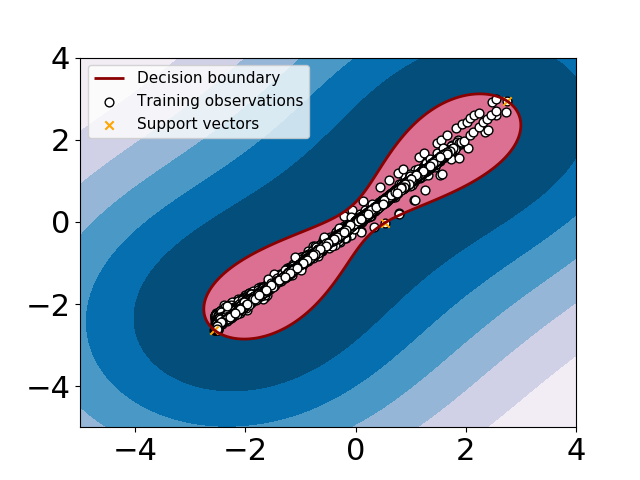
\includegraphics[width = .7\textwidth]{report/figures/analysis/gridsearch/Novelty detection, 4 training, gamma = 0.05 nu = 0.00021166260979997884.png}
        \caption{$\gamma = 0.05$, $\nu = 2/N$. score $=0.960$}
        \label{fig:my_label}
    \end{figure}
    
    \begin{figure}
        \centering
        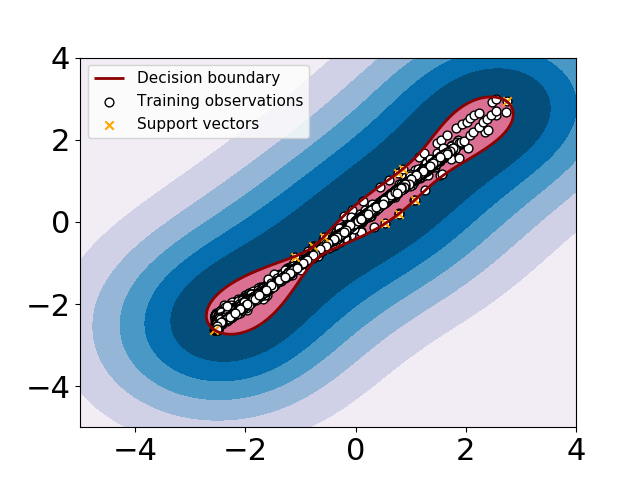
\includegraphics[width = .7\textwidth]{report/figures/analysis/gridsearch/Novelty detection, 5 training, gamma = 0.2 nu = 0.00010583130489998942.png}
        \caption{$\gamma = 0.2$, $\nu = 1/N$. score $=0.957$}
        \label{fig:my_label}
    \end{figure}
    
    
    \begin{figure}
        \centering
        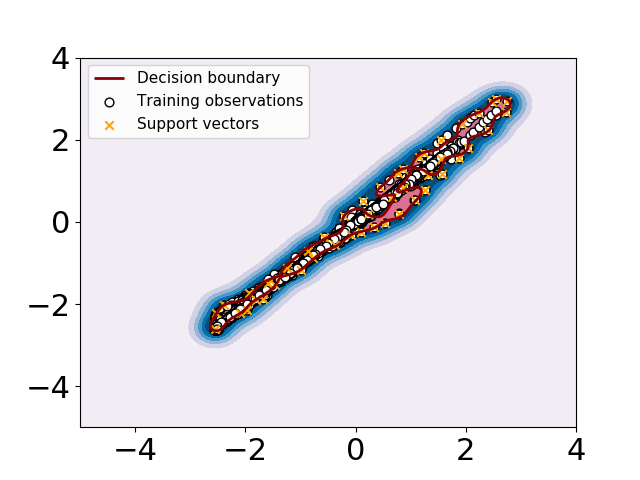
\includegraphics[width = .7\textwidth]{report/figures/analysis/gridsearch/Novelty detection, -5 training, gamma = 8 nu = 1.0583130489998942e-05.png}
        \caption{$\gamma = 8$, $\nu = 1/10N5$. score $=-44.437$}
        \label{fig:my_label}
    \end{figure}
    
    \begin{figure}
        \centering
        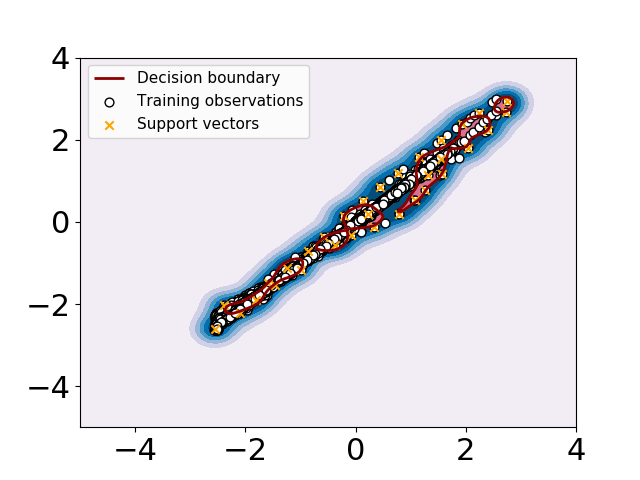
\includegraphics[width = .7\textwidth]{report/figures/analysis/gridsearch/Novelty detection, -4 training, gamma = 8 nu = 4.233252195999577e-06.png}
        \caption{$\gamma = 8$, $\nu = 1/25N$. score $=-51.780$}
        \label{fig:my_label}
    \end{figure}
    
    \begin{figure}
        \centering
        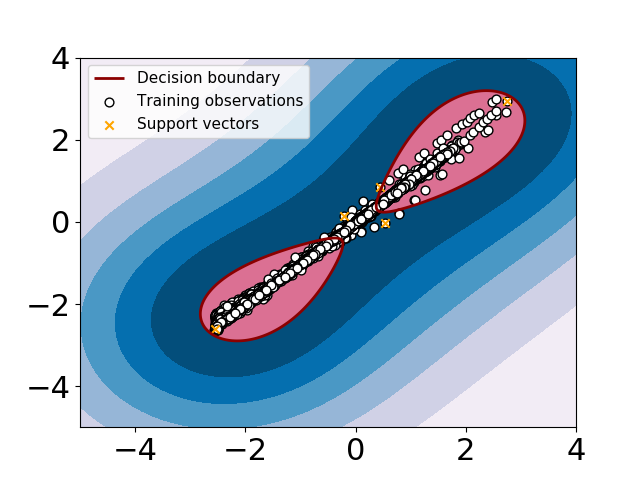
\includegraphics[width = .7\textwidth]{report/figures/analysis/gridsearch/Novelty detection, -3 training, gamma = 0.1 nu = 4.233252195999577e-06.png}
        \caption{$\gamma = 0.1$, $\nu = 1/25N$. score $=-57.461$}
        \label{fig:my_label}
    \end{figure}
    
    
    \begin{figure}
        \centering
        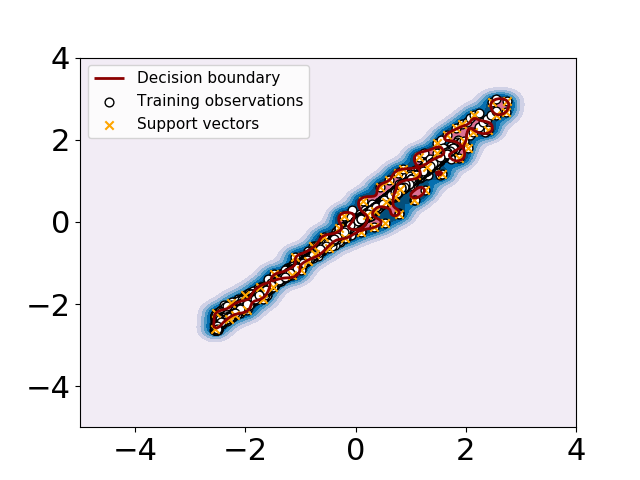
\includegraphics[width = .7\textwidth]{report/figures/analysis/gridsearch/Novelty detection, -2 training, gamma = 16 nu = 1.0583130489998942e-05.png}
        \caption{$\gamma = 16$, $\nu = 1/10N$. score $=-71.082$}
        \label{fig:my_label}
    \end{figure}
    
    
    \begin{figure}
        \centering
        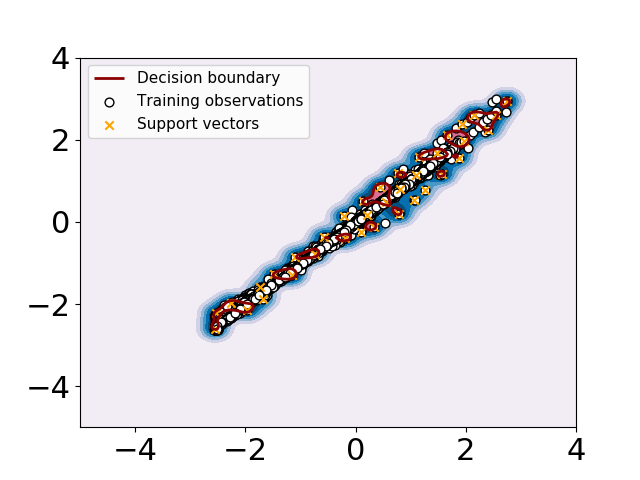
\includegraphics[width = .7\textwidth]{report/figures/analysis/gridsearch/Novelty detection, -1 training, gamma = 16 nu = 4.233252195999577e-06.png}
        \caption{$\gamma = 16$, $\nu = 1/25N$. score $=-506.263$}
        \label{fig:my_label}
    \end{figure}

\chapter{LSTM gridsearch}\label{appendix:lstm_grid}
    The model history for the training of the five best and five worst LSTM configurations are plotted below, from best to worst. As can be seen the worst configurations are stopped after only a few epochs due to lack of improvement of the predictions of the network. 
    \begin{figure}
        \begin{minipage}[b]{0.49\linewidth}
            \centering
            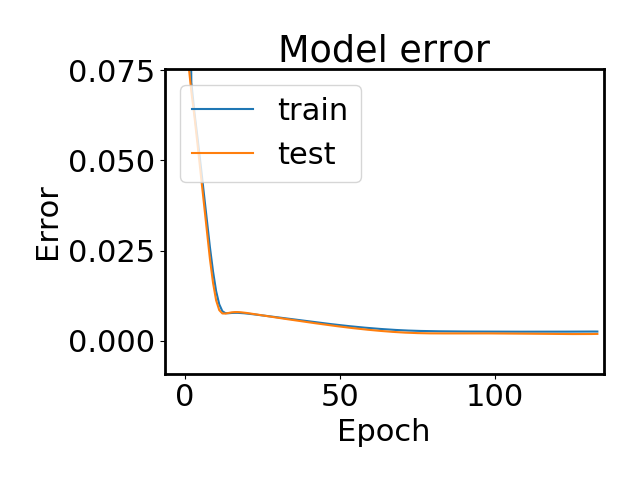
\includegraphics[width = \textwidth]{report/figures/analysis/lstm_gridsearch/best_lstm_error_zoomed.png}
            \caption{Training history for the best LSTM configuration}
            \label{fig:lstm_grid_error_best_appendix}
        \end{minipage}
        \hfill\vline\hfill
        \begin{minipage}[b]{0.49\linewidth}
            \centering
            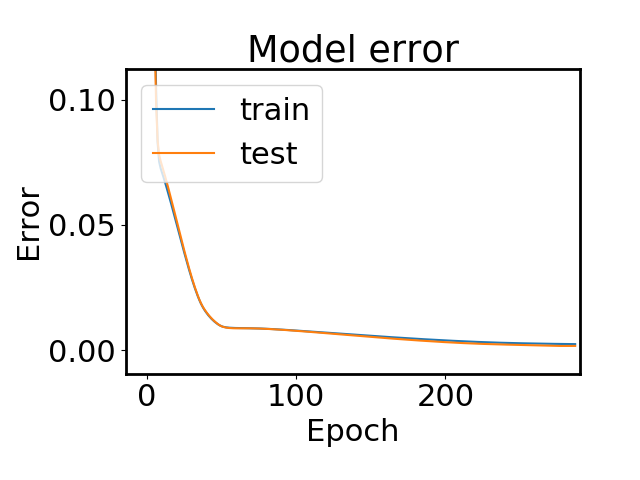
\includegraphics[width = \textwidth]{report/figures/analysis/lstm_gridsearch/best_lstm_error_2_zoomed.png}
            \caption{Training history for the second best LSTM configuration}
            \label{fig:lstm_grid_error_worst_appendix}
        \end{minipage}
    \end{figure}

    \begin{figure}
        \begin{minipage}[b]{0.49\linewidth}
            \centering
            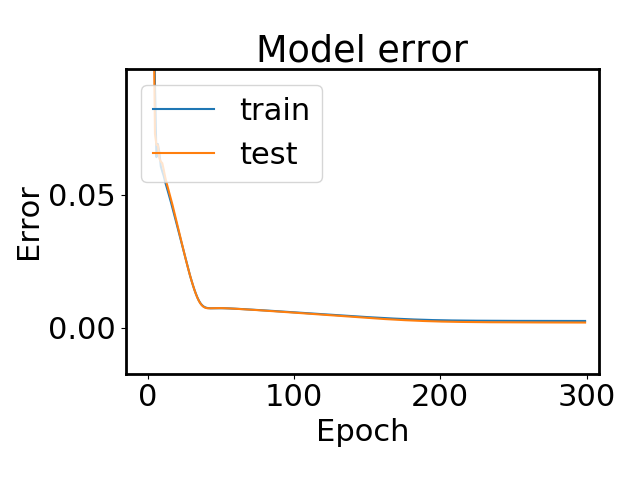
\includegraphics[width = \textwidth]{report/figures/analysis/lstm_gridsearch/best_lstm_error_3_zoomed.png}
            \caption{Training history for the third best LSTM configuration}
            \label{fig:lstm_grid_error_best_appendix}
        \end{minipage}
        \hfill\vline\hfill
        \begin{minipage}[b]{0.49\linewidth}
            \centering
            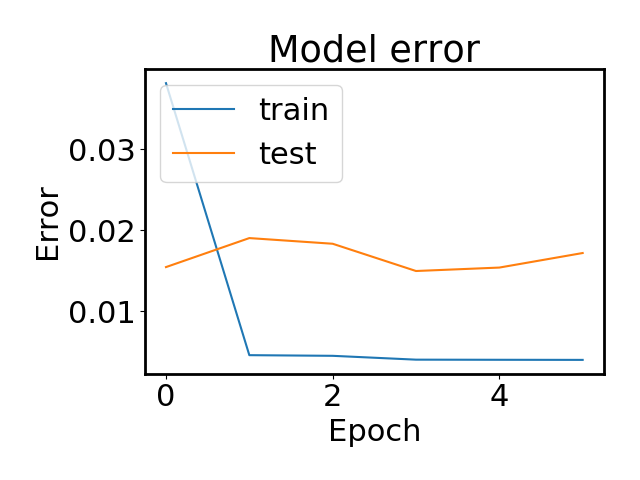
\includegraphics[width = \textwidth]{report/figures/analysis/lstm_gridsearch/worst_lstm_error_-3.png}
            \caption{Training history for the fourth best LSTM configuration}
            \label{fig:lstm_grid_error_worst_appendix}
        \end{minipage}
    \end{figure}

    \begin{figure}
        \begin{minipage}[b]{0.49\linewidth}
            \centering
            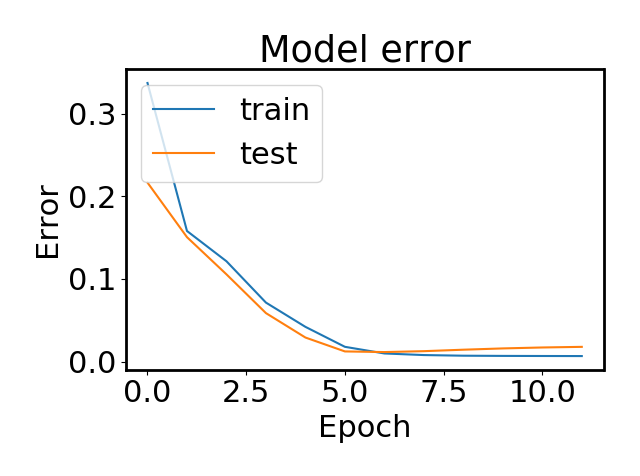
\includegraphics[width = \textwidth]{report/figures/analysis/lstm_gridsearch/worst_lstm_error_-5.png}
            \caption{Training history for the fifth worst LSTM configuration}
            \label{fig:lstm_grid_error_best_appendix}
        \end{minipage}
        \hfill\vline\hfill
        \begin{minipage}[b]{0.49\linewidth}
            \centering
            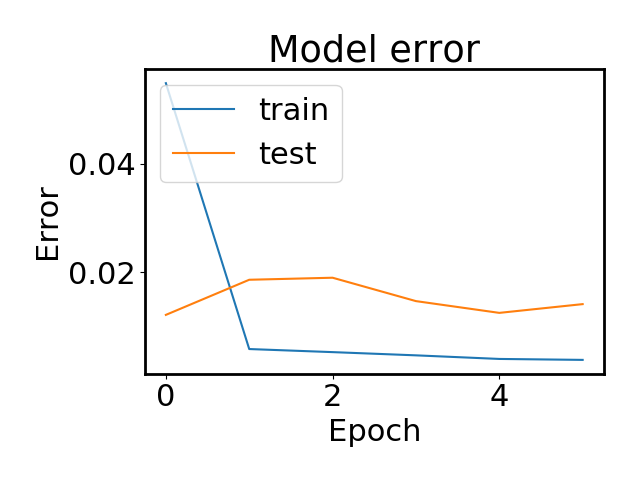
\includegraphics[width = \textwidth]{report/figures/analysis/lstm_gridsearch/worst_lstm_error_-4.png}
            \caption{Training history for the fourth worst LSTM configuration}
            \label{fig:lstm_grid_error_worst_appendix}
        \end{minipage}
    \end{figure}

    \begin{figure}
        \begin{minipage}[b]{0.49\linewidth}
            \centering
            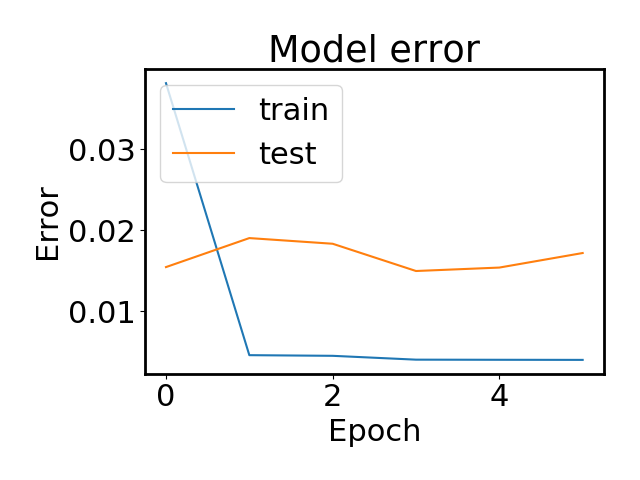
\includegraphics[width = \textwidth]{report/figures/analysis/lstm_gridsearch/worst_lstm_error_-3.png}
            \caption{Training history for the third worst LSTM configuration}
            \label{fig:lstm_grid_error_best_appendix}
        \end{minipage}
        \hfill\vline\hfill
        \begin{minipage}[b]{0.49\linewidth}
            \centering
            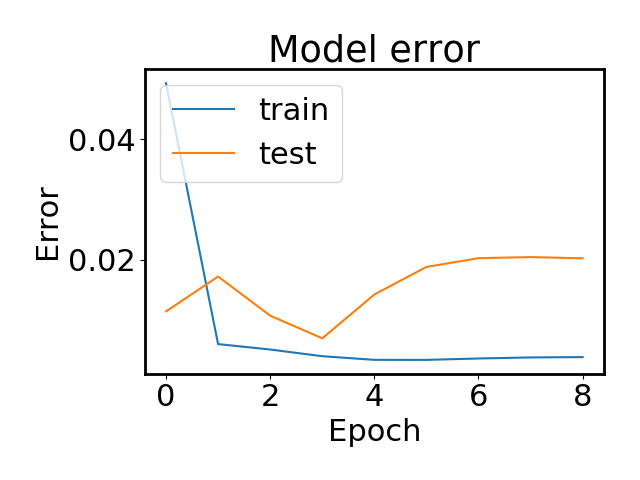
\includegraphics[width = \textwidth]{report/figures/analysis/lstm_gridsearch/worst_lstm_error_-2.png}
            \caption{Training history for the second worst LSTM configuration}
            \label{fig:lstm_grid_error_worst_appendix}
        \end{minipage}
    \end{figure}
    
    \begin{figure}
        \begin{minipage}[b]{0.45\linewidth}
            \centering
            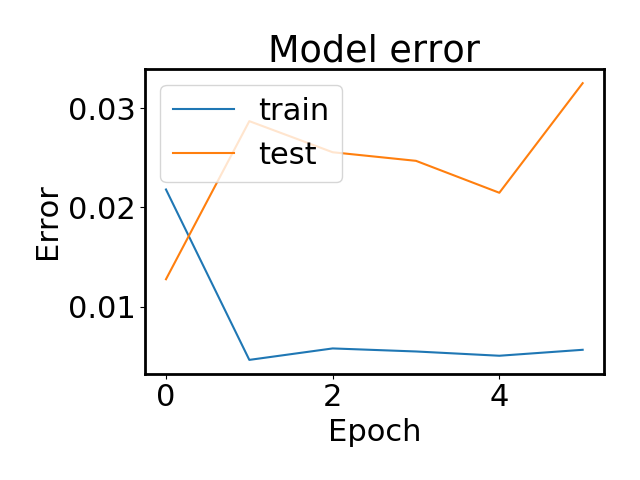
\includegraphics[width = \textwidth]{report/figures/analysis/lstm_gridsearch/worst_lstm_error_-1.png}
            \caption{Training history for the worst LSTM configuration}
            \label{fig:lstm_grid_error_best_appendix}
        \end{minipage}
    \end{figure}

% \chapter{SVM gridsearch plant 2}
%     A gridsearch after the optimal hyperparameterization for the one class SVM when trained on data from plant 2 is performed. The result is presented in table \ref{tab:svm_gridsearch2}, and the decision boundaries for the two best and two worst parameterizations are seen below. 
%     \begin{table}[h]
%         \centering
%         \begin{tabular}{|c|c|c|}
%             \hline
%              Score  &   $\gamma$    & $\nu$         \\ \hline
%              0.995  &   $0.05$      & $\frac{1}{5N}$ \\ \hline
%              0.987  &   $0.05$      & $\frac{1}{2N}$ \\ \hline
%              0.975  &   $0.05$      & $\frac{1}{N}$ \\ \hline
%              0.972  &   $0.04$      & $\frac{}{10N}$ \\ \hline
%              0.970  &   $0.03$      & $\frac{1}{10N}$ \\ \hline
%              -50.698  &   $10$      & $\frac{1}{10N}$ \\ \hline
%              -91.291  &   $1$      & $\frac{1}{10N}$ \\ \hline
%              -94.296  &   $10$      & $\frac{1}{25N}$ \\ \hline
%              -124.473  &  $0.8$      & $\frac{1}{10N}$ \\ \hline
%              -193.239  &  $5$      & $\frac{1}{25N}$ \\ \hline
             
%         \end{tabular}
%         \caption{Table showing the five best and five worst scores for the gridsearch after optimal hyperparameters for the one class SVM. $N = $ number of samples.}
%         \label{tab:svm_gridsearch2}
%     \end{table}
        
%         \begin{figure}
%             \centering
%             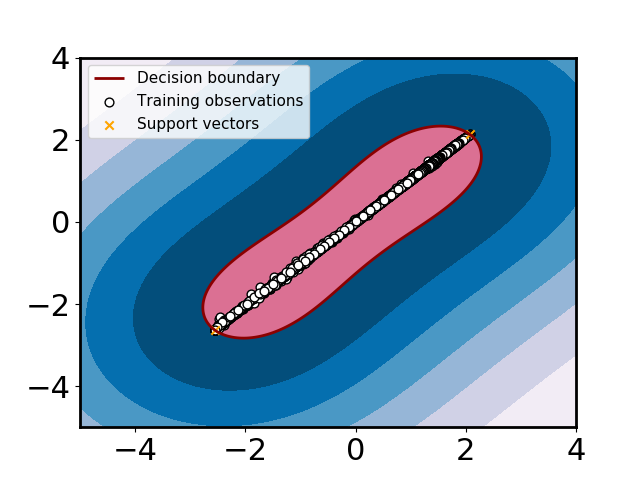
\includegraphics[width = .7\textwidth]{report/figures/analysis/gridsearchPlant2/Novelty detection training, gamma = 0.05 nu = 1.554001554001554e-05.png}
%             \caption{Score = 0.995, #1}
%             \label{fig:my_label}
%         \end{figure}
    
%         \begin{figure}
%             \centering
%             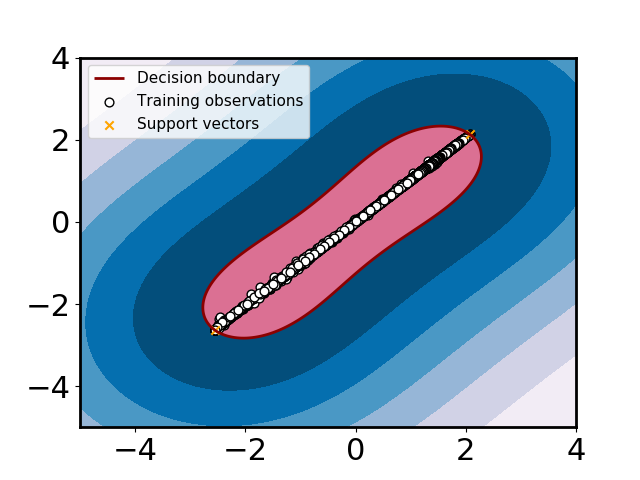
\includegraphics[width = .7\textwidth]{report/figures/analysis/gridsearchPlant2/Novelty detection training, gamma = 0.05 nu = 3.885003885003885e-05.png}
%             \caption{Score = .987, #2}
%             \label{fig:my_label}
%         \end{figure}
        
%         \begin{figure}
%             \centering
%             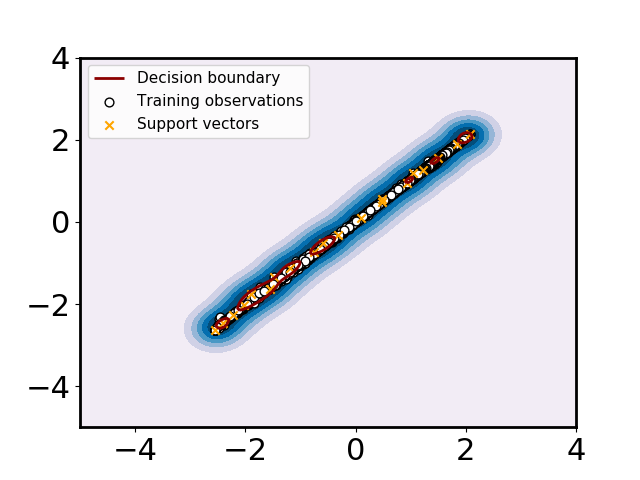
\includegraphics[width = .7\textwidth]{report/figures/analysis/gridsearchPlant2/Novelty detection training, gamma = 5 nu = 3.108003108003108e-06.png}
%             \caption{Score = -193.239, worst}
%             \label{fig:my_label}
%         \end{figure}
    
%         \begin{figure}
%             \centering
%             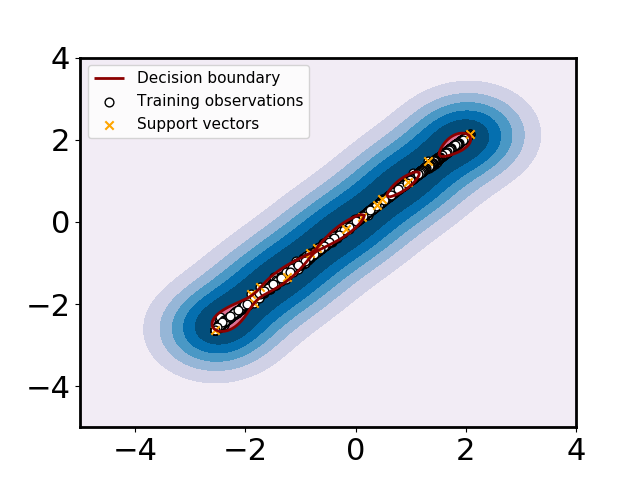
\includegraphics[width = .7\textwidth]{report/figures/analysis/gridsearchPlant2/Novelty detection training, gamma = 1 nu = 7.77000777000777e-06.png}
%             \caption{Score = -124.473 second to last wors}
%             \label{fig:my_label}
%         \end{figure}
        
        

\chapter{Training case 1}\label{appendix:training_case1}
    Additional plots from analysis of training case 1 is presented below. 
    \begin{figure}
        \centering
        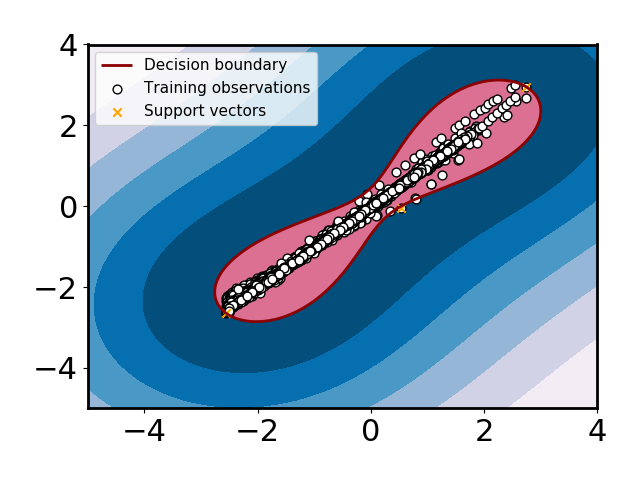
\includegraphics[width=0.7\textwidth]{report/figures/analysis/plant1_training/svm_boundary.png}
        \caption{Decision boundary for the one class SVM classifier. Support vectors and training observations are plotted. All samples located outside the red boundary are classified as anomalies.}
        \label{fig:svm_train_p1_boundary}
    \end{figure}
    
    
     \begin{figure}
        \centering
        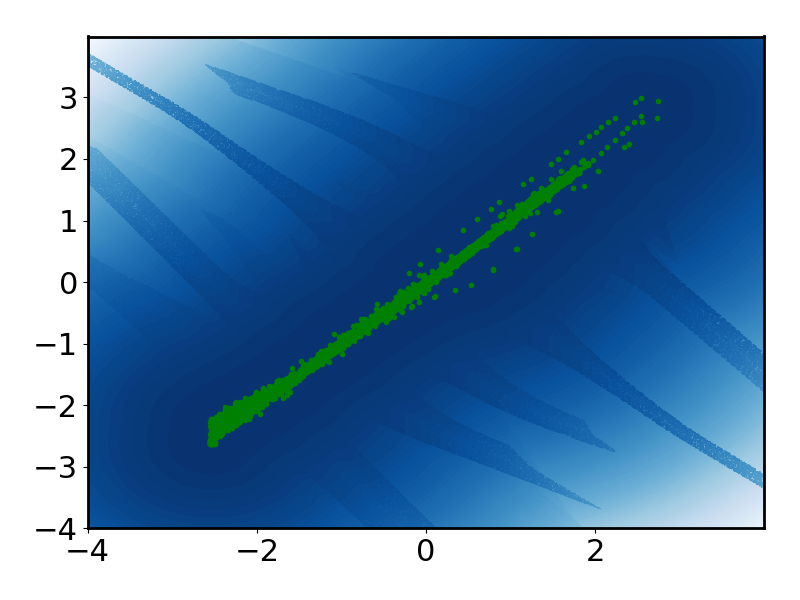
\includegraphics[width=0.7\textwidth]{report/figures/analysis/plant1_training/kde_boundary.png}
        \caption{The KDE anomaly scorers probability score plotted as contours in the space of the scaled training data. Traning samples are seen in green. As the grid value becomes more and more anomalous the color becomes lighter.}
        \label{fig:my_label}
    \end{figure}
    
    
    \begin{figure}
        \centering
        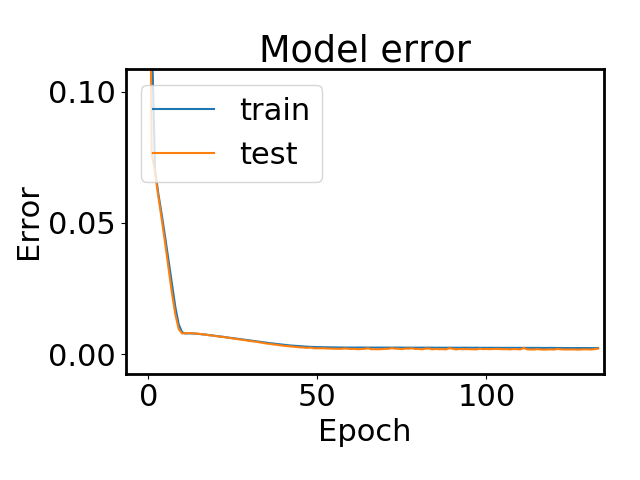
\includegraphics[width=0.7\textwidth]{report/figures/analysis/plant1_training/lstm_model_error.png}
        \caption{Model error for the LTSM network as the number of epochs increase.}
        \label{fig:lstm_training_plant1}
    \end{figure}
    
    \begin{figure}
        \centering
        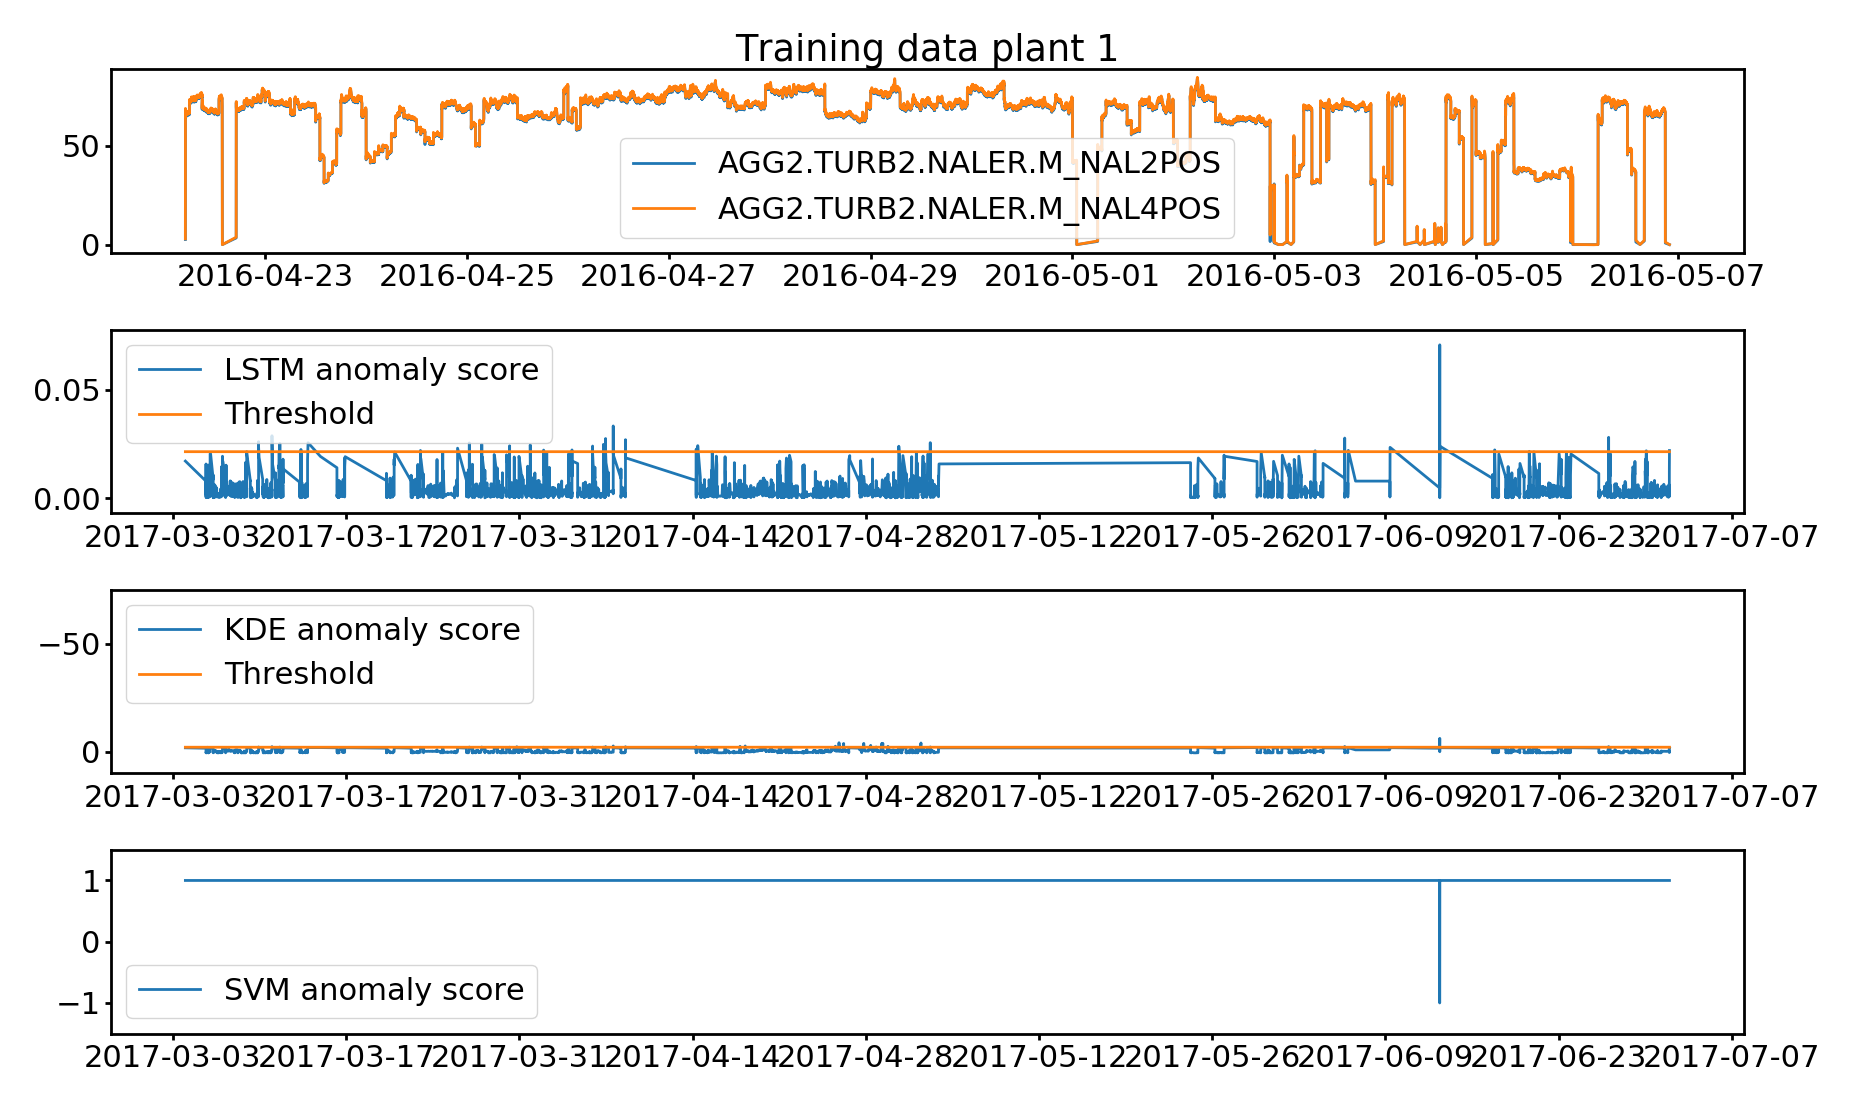
\includegraphics[width=\textwidth]{report/figures/analysis/plant1_training/training_data_anomaly.png}
        \caption{Anomaly score for training set for training case 1.As can be seen the anomaly scores for the KDE and LSTM anomaly scorers are much lower than for the production and artificial data seen in the analysis. One datapoint is classified as an outlier by the one class SVM classifier, it is also given a higher anomaly score by the scorers.}
        \label{fig:anomaly_training_plant1_case1}
    \end{figure}
    
    \begin{figure}
        \centering
        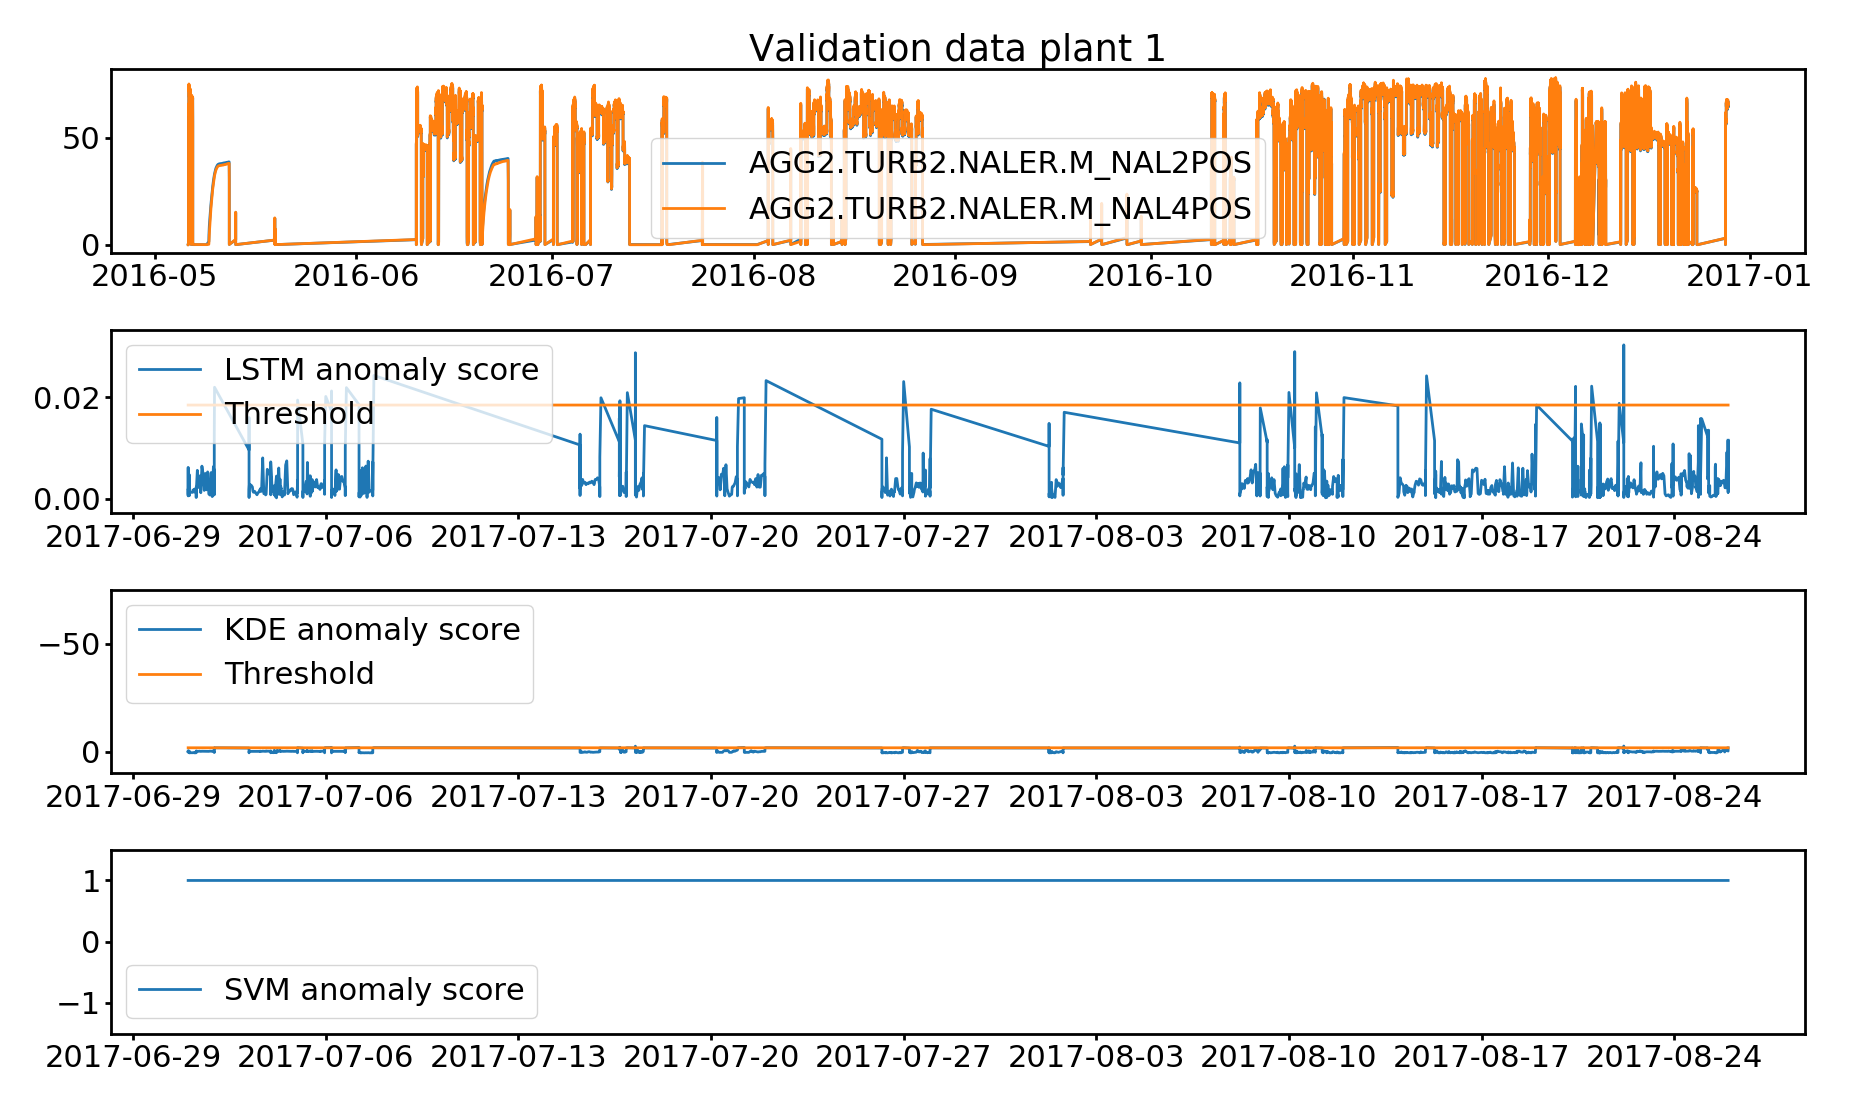
\includegraphics[width=\textwidth]{report/figures/analysis/plant1_training/test_data_anomaly.png}
        \caption{Anomaly score for validation set for training case 1. As can be verified very low anomaly scores are seen for both the KDE and LSTM anomaly scorers, the one class SVM anomaly classifier correctly classifies all samples as normal.}
        \label{fig:anomaly_training_plant1}
    \end{figure}

% \chapter{Training case 2}
%     \begin{figure}
%         \centering
%         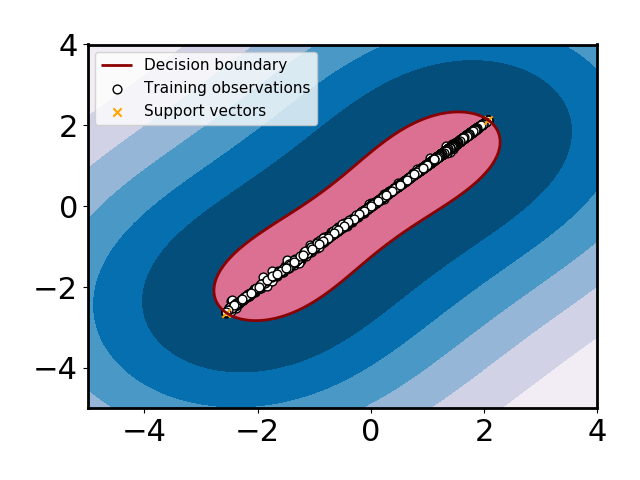
\includegraphics[width=0.7\textwidth]{report/figures/analysis/plant2_train_short/svm_boundary.png}
%         \caption{one class svm boundary after training on data from plant 1 after the incident}
%         \label{fig:svm_train_p1_boundary}
%     \end{figure}
    
    
%      \begin{figure}
%         \centering
%         \includegraphics[width=0.7\textwidth]{report/figures/analysis/plant2_train_short/kde_boundary.png}
%         \caption{KDE boundary based on probability score, training data seen in green.}
%         \label{fig:my_label}
%     \end{figure}
    
    
%     \begin{figure}
%         \centering
%         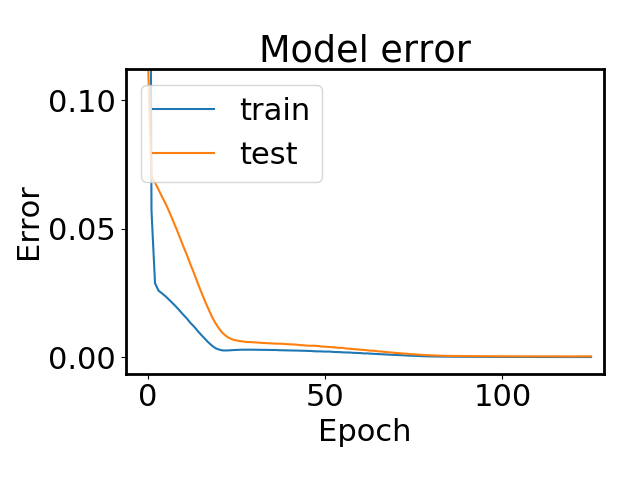
\includegraphics[width=0.7\textwidth]{report/figures/analysis/plant2_train_short/lstm_model_error.png}
%         \caption{Learning rate for lstm at plant 1 training after incident}
%         \label{fig:lstm_training_plant1}
%     \end{figure}
    
%     \begin{figure}
%         \centering
%         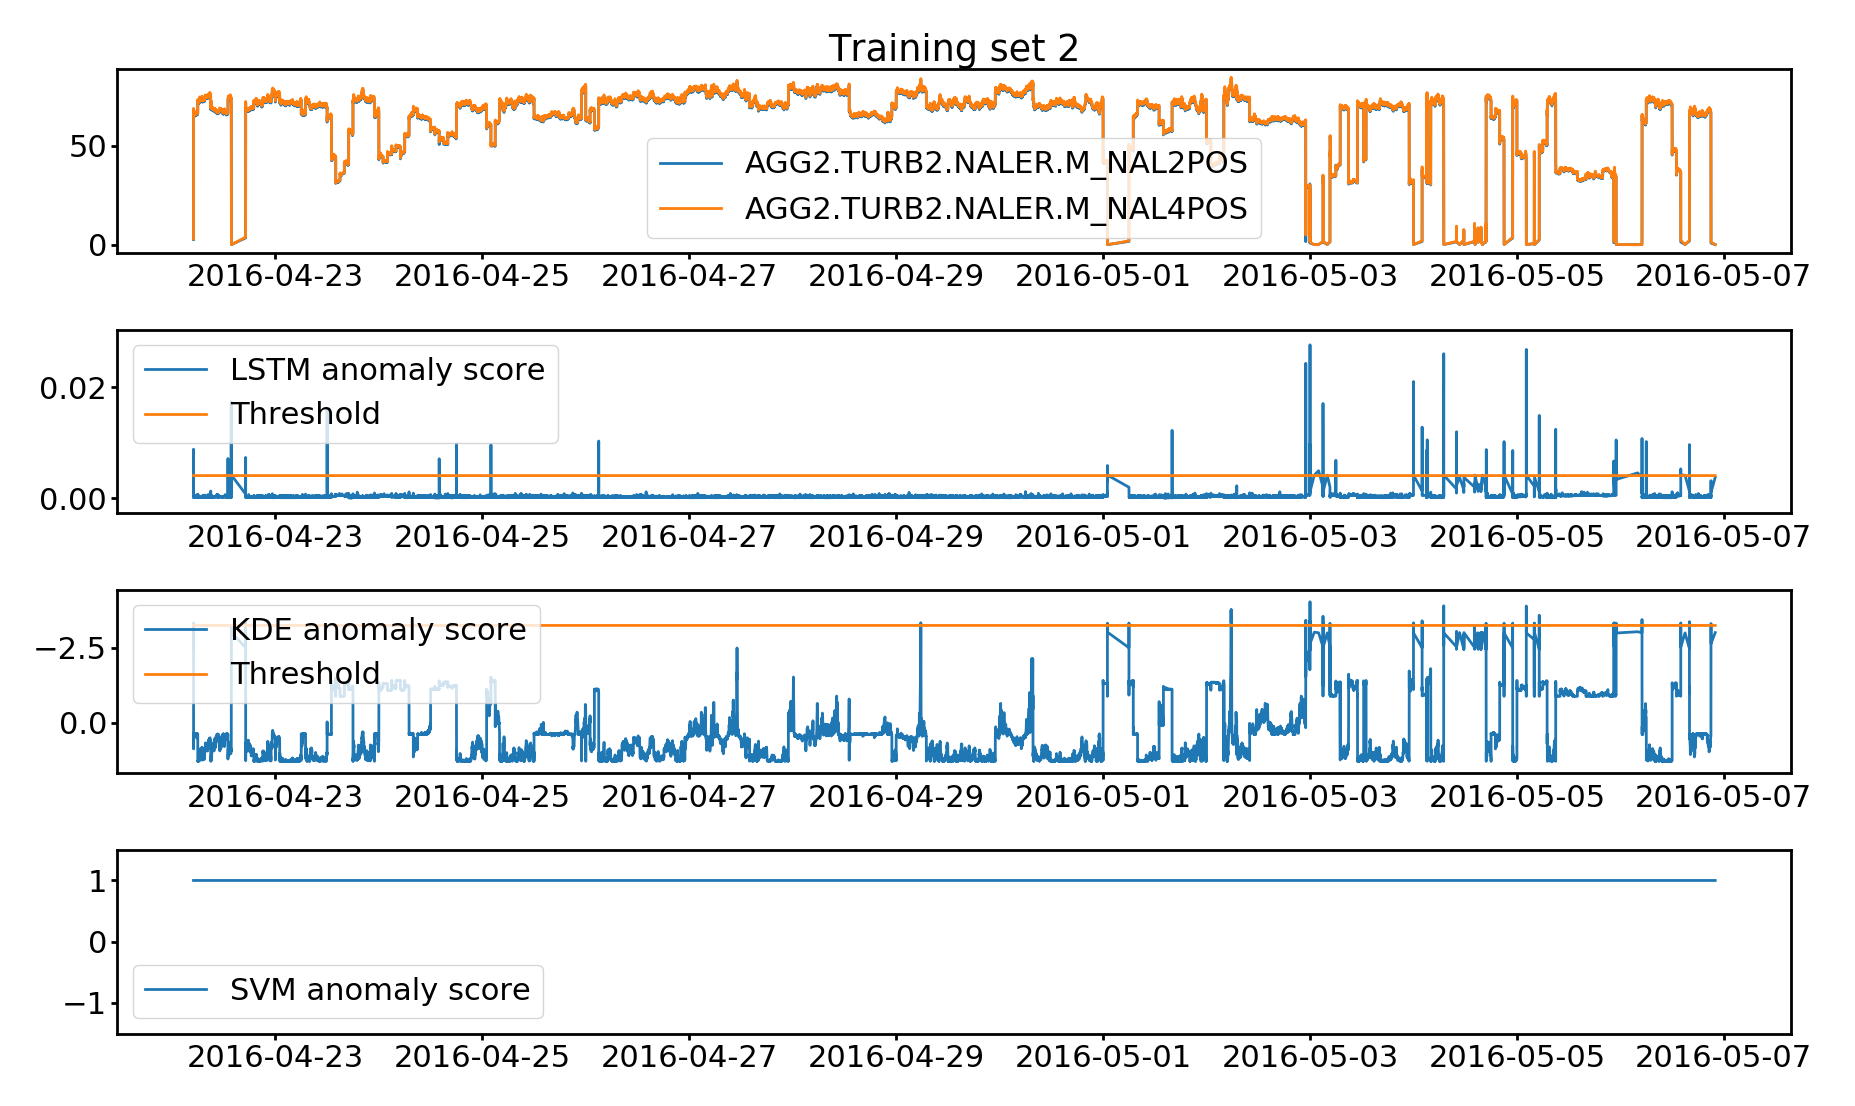
\includegraphics[width=\textwidth]{report/figures/analysis/plant2_train_short/training_data_anomaly.png}
%         \caption{Anomaly score for training set at plant 1.}
%         \label{fig:anomaly_training_plant1}
%     \end{figure}

%     \begin{figure}
%         \centering
%         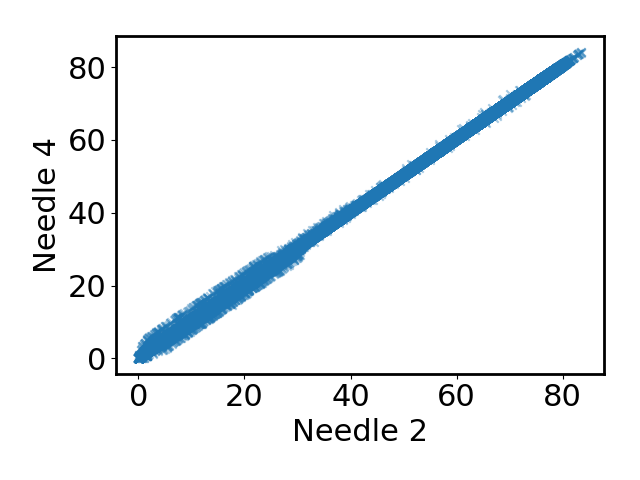
\includegraphics[width=\textwidth]{report/figures/analysis/plant2_train_long/needle_scatterplots.png}
%         \caption{Scatterplot for needles}
%         \label{fig:anomaly_training_plant1}
%     \end{figure}

    
\chapter{Training case 3}
    \begin{figure}
        \centering
        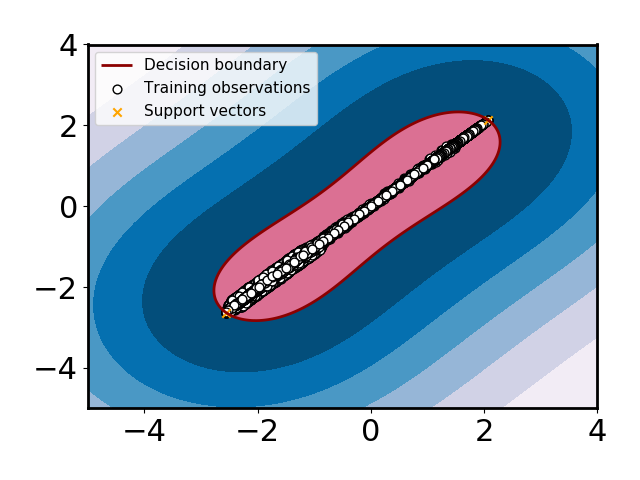
\includegraphics[width=0.7\textwidth]{report/figures/analysis/plant2_train_long/svm_boundary.png}
        \caption{one class svm boundary after training on data from plant 1 after the incident}
        \label{fig:svm_train_p1_boundary}
    \end{figure}
    
    
     \begin{figure}
        \centering
        \includegraphics[width=0.7\textwidth]{report/figures/analysis/plant2_train_long/kde_boundary.png}
        \caption{KDE boundary based on probability score, training data seen in green.}
        \label{fig:my_label}
    \end{figure}
    
    
    \begin{figure}
        \centering
        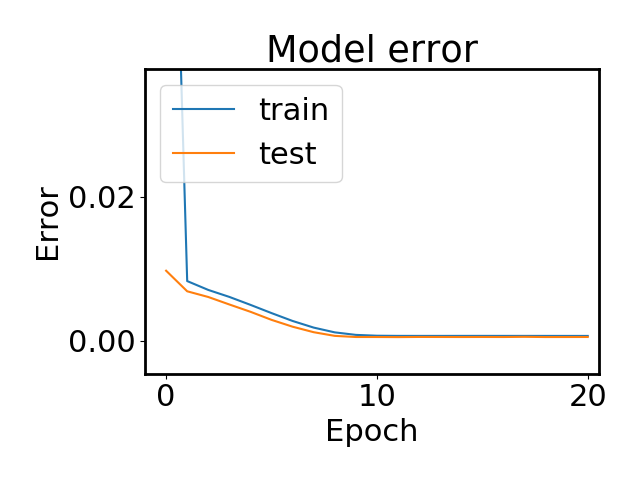
\includegraphics[width=0.7\textwidth]{report/figures/analysis/plant2_train_long/lstm_model_errror.png}
        \caption{Learning rate for lstm at plant 1 training after incident}
        \label{fig:lstm_training_plant1}
    \end{figure}
    
    \begin{figure}
        \centering
        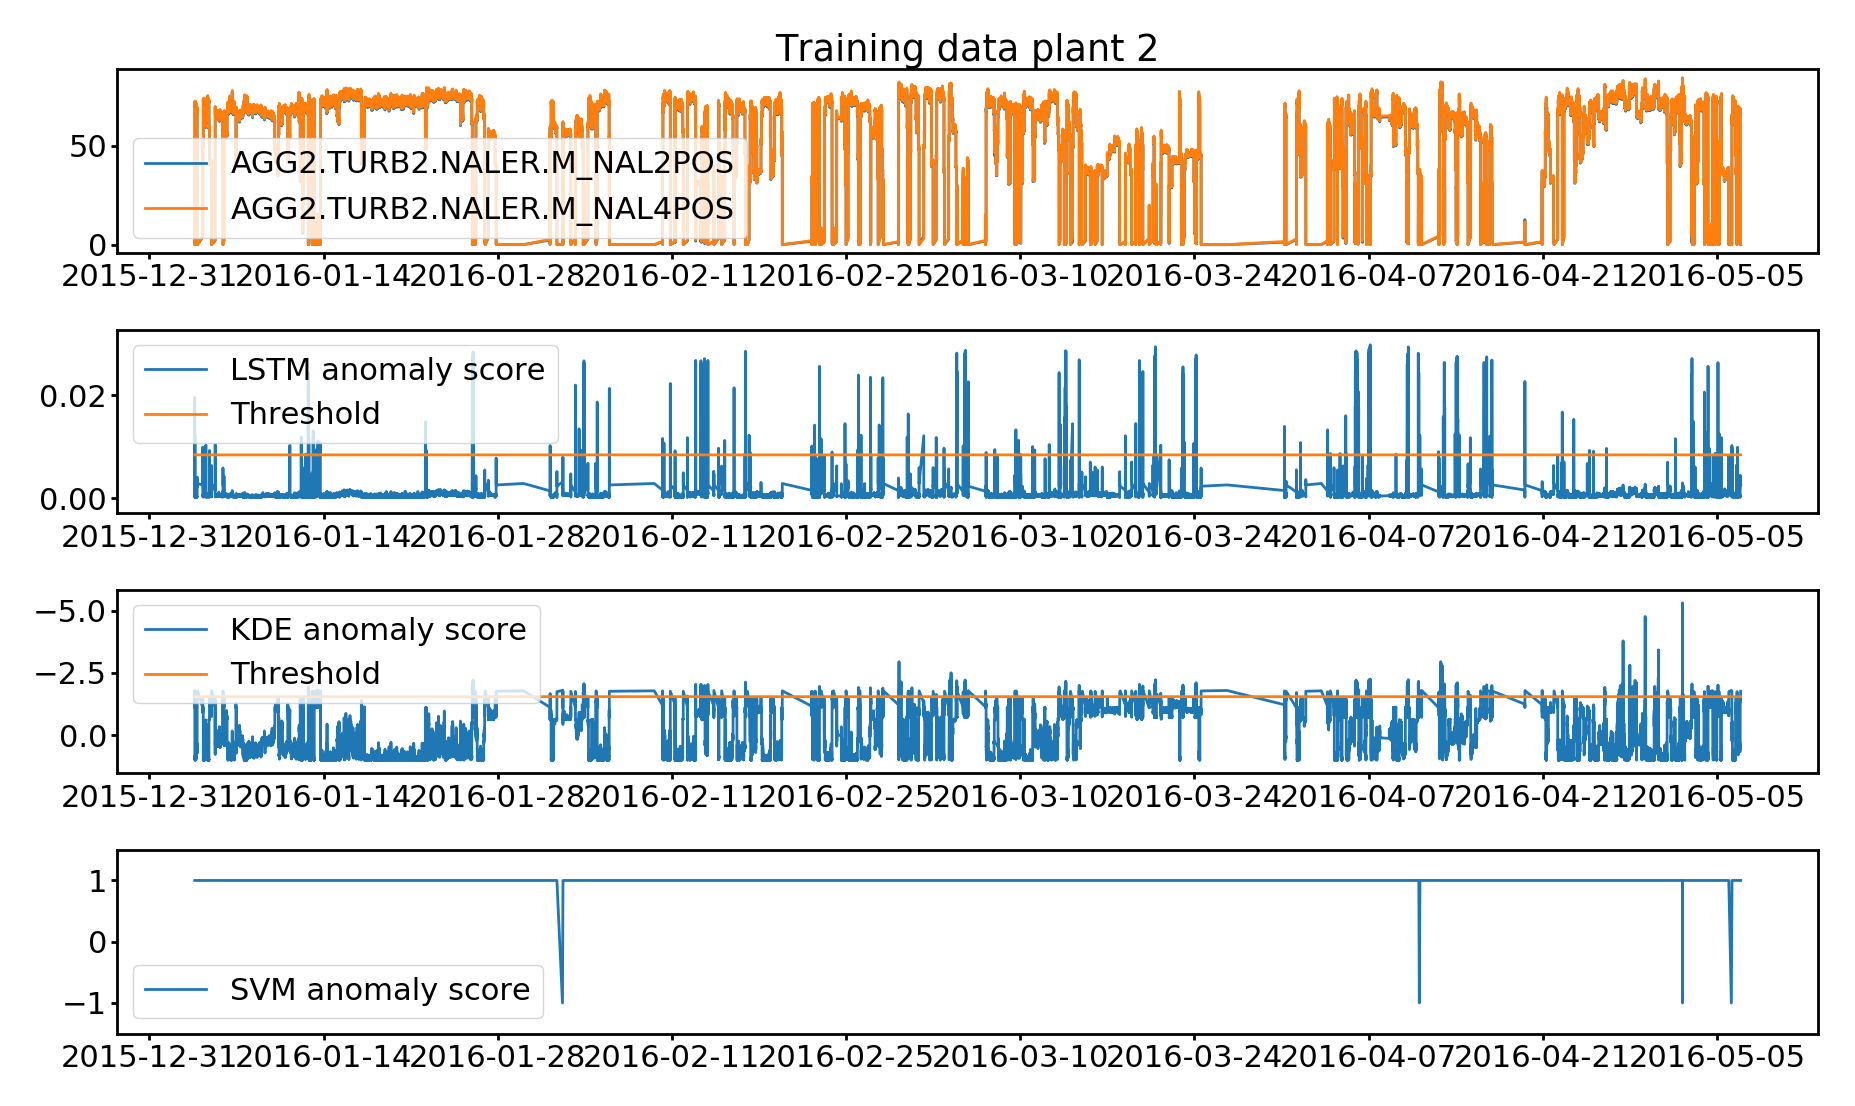
\includegraphics[width=\textwidth]{report/figures/analysis/plant2_train_long/training_data_anomaly.png}
        \caption{Anomaly score for training set at plant 1.}
        \label{fig:anomaly_training_plant1}
    \end{figure}
    
    \begin{figure}
        \centering
        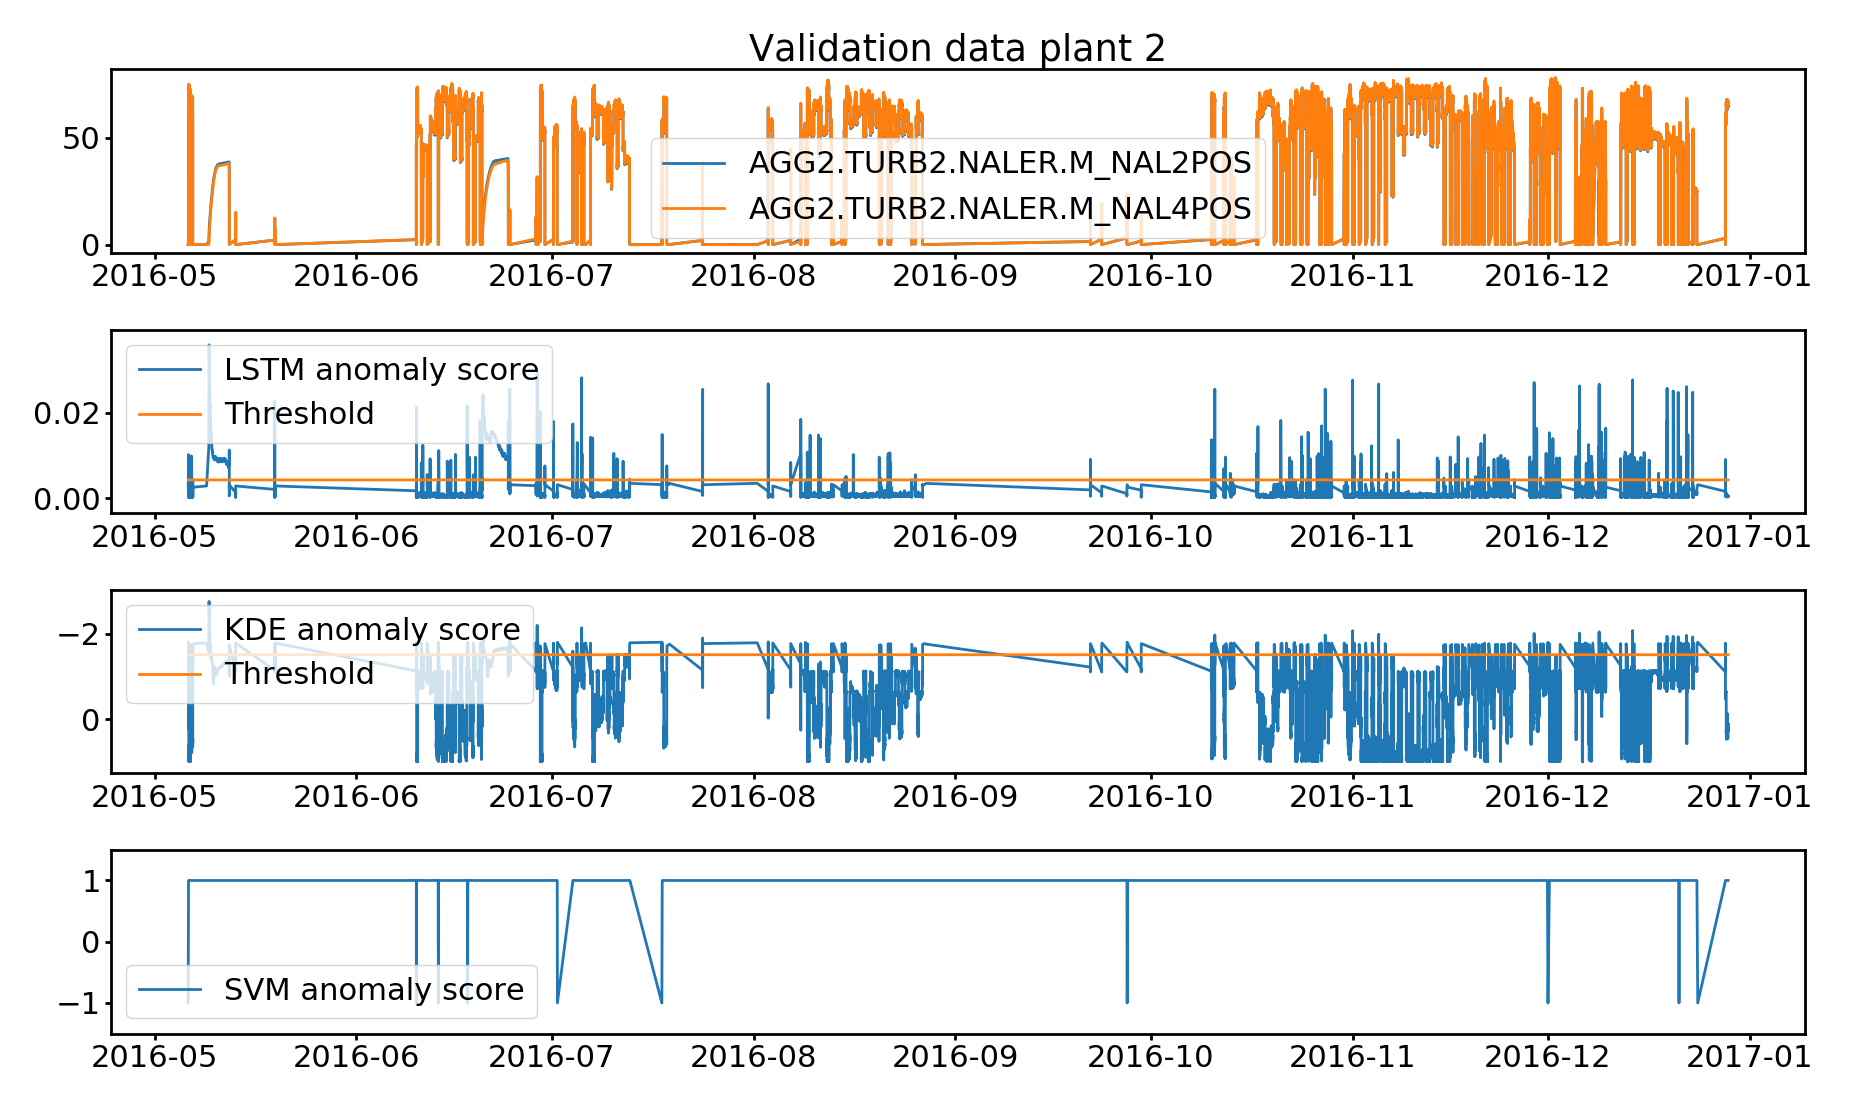
\includegraphics[width=\textwidth]{report/figures/analysis/plant2_train_long/test_data_anomaly.png}
        \caption{Anomaly score for training set at plant 1.}
        \label{fig:anomaly_training_plant1}
    \end{figure}
    
    \begin{figure}
        \centering
        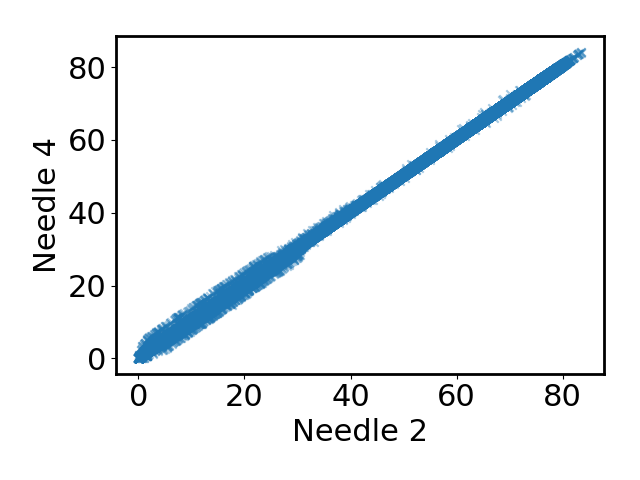
\includegraphics[width=\textwidth]{report/figures/analysis/plant2_train_long/needle_scatterplots.png}
        \caption{Scatterplot for needles}
        \label{fig:anomaly_training_plant1}
    \end{figure}